\chapter{Using the CPNGenerator Interpreter}

Once the component business logic operations are modeled, it is time to generate an analysis model for the application. 

\emph{Reminder:} In order for this section to be useful, a clean installation of the CPN Tools 4 Tool Suite is required. 

From the Software Deployment aspect in the F6ML model, click on the CPNGenerator interpreter (Figure \ref{fig:interpreter}).

\begin{figure}[ht]
\centering
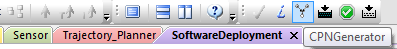
\includegraphics[width=0.80\textwidth]{./figs/interpreter}
\caption{CPNGenerator Interpreter}
\label{fig:interpreter}
\vspace{-0.2in}
\end{figure}
\vspace{0.1in} 

Once the interpreter starts, it prints a sequence of debug messages. These messages are organized as follows: 

\subsection{Application Summary}

For every application, the first set of debug messages shows the following messages for each component: 
\begin{itemize}
\item Component Name, Actor Name, Actor ID, Actor Priority, Node Name
\item Receptacle (if any) Name, Interface Name, Type of Receptacle
\item Facet (if any) Name, Interface Name
\item DDS Publisher Name, Topic Name
\item DDS Subscriber Name, Topic Name, Subscription Type
\end{itemize}

Figure \ref{fig:app_summary_1} shows the application summary for the Trajectory Planning Application: 

\begin{figure}[ht]
\centering
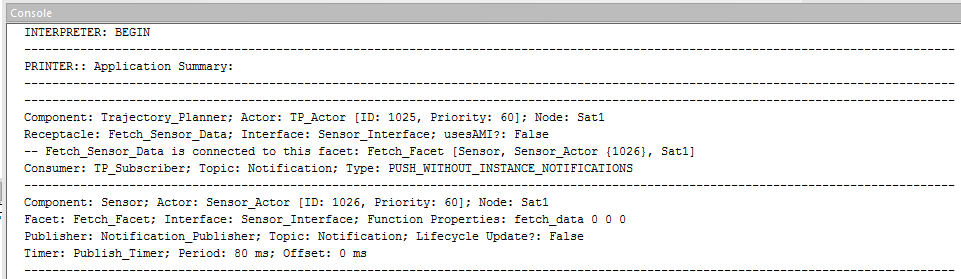
\includegraphics[width=0.99\textwidth]{./figs/app_summary_1}
\caption{Application Summary}
\label{fig:app_summary_1}
\vspace{-0.2in}
\end{figure}
\vspace{0.1in} 

\begin{figure}[ht]
\centering
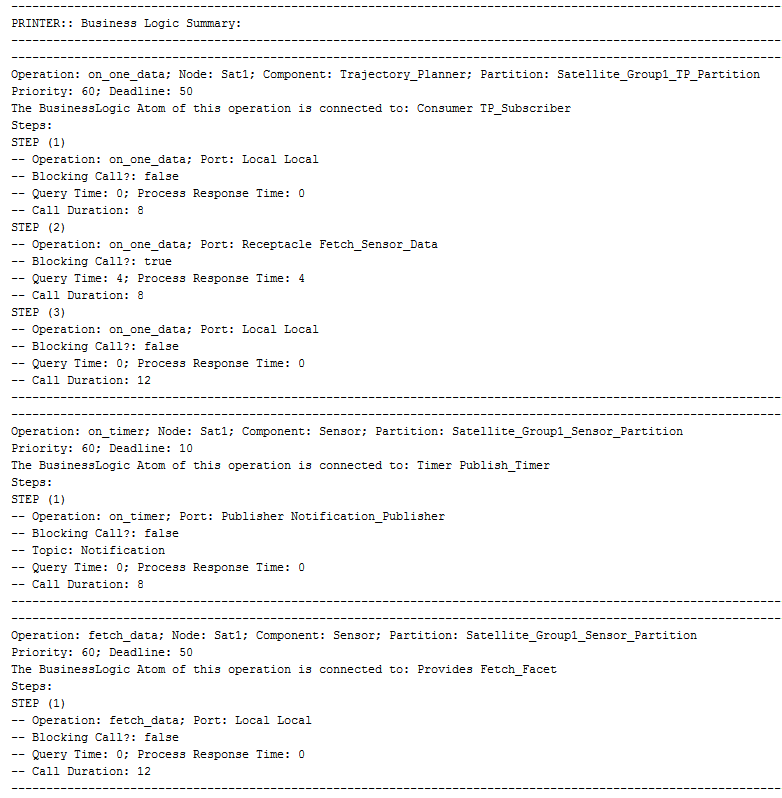
\includegraphics[width=0.8\textwidth]{./figs/app_summary_2}
\caption{Business Logic Summary}
\label{fig:app_summary_2}
\vspace{-0.2in}
\end{figure}
\vspace{0.1in} 

\subsection{Business Logic Summary}
The second set of debug messages shows the summary of every component operation BusinessLogic in the application. This includes: 
\begin{itemize}
\item Operation Name, Node Name, Component Name, Partition Name.
\item Operation Priority, Operation Deadline.
\item Set of Steps in the Component Operation.
\end{itemize}

\newpage

\subsection{Generated CPN files}

The CPNGenerator generates two files for the timing analysis. 
\begin{itemize}
\item CPN\_Analysis\_Model.cpn
\item functions.sml
\end{itemize}

The CPN\_Analysis\_Model.cpn is the main colored petri net file. This is the primary analysis model. The extension .cpn refers to a CPN Tools-based colored petri net. This model is therefore opened by CPN Tools. 

\begin{figure}[ht]
\centering
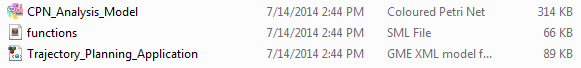
\includegraphics[width=0.9\textwidth]{./figs/generated}
\label{fig:generated}
\vspace{-0.2in}
\end{figure}
\vspace{0.1in} 

In addition, the functions.sml file is standard ML file that contains all of the functions used by transition guards and arc inscriptions in the CPN model.

\begin{figure}[ht]
\centering
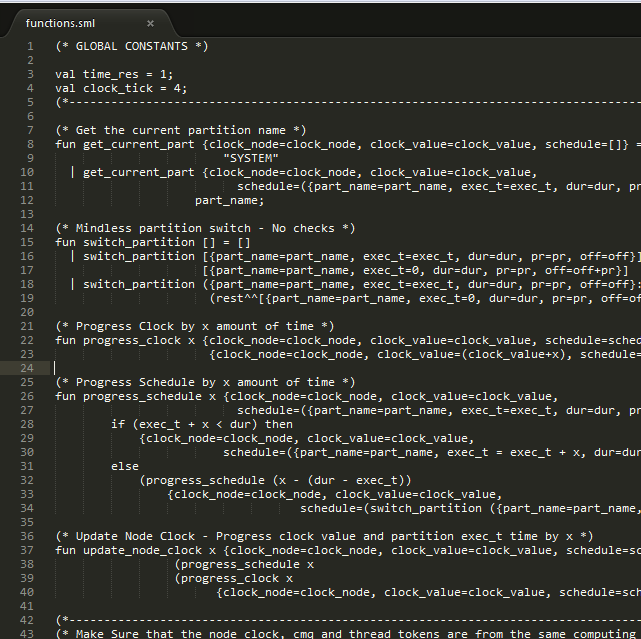
\includegraphics[width=0.9\textwidth]{./figs/functions}
\label{fig:functions}
\vspace{-0.2in}
\end{figure}
\vspace{0.1in} 



